\chapter{Methods}


\section{Design}
%-------------------------------------------%

The project consists of several core components: a SerpentAI game agent plugin, a dataset management program, a frame-action synchronizer, a replay parser, and a machine learning program.

The first phase of the project is data preprocessing. This consists of converting the plaintext replay files into a labeled dataset. The dataset management program is used to move all of the replay files into folders corresponding with their game versions. This results in the following directory structure:

%% Source: https://tex.stackexchange.com/a/270761
\begin{forest}
    for tree={
        font=\ttfamily,
        grow'=0,
        child anchor=west,
        parent anchor=south,
        anchor=west,
        calign=first,
        edge path={
            \noexpand\path [draw, \forestoption{edge}]
            (!u.south west) +(7.5pt,0) |- node[fill,inner sep=1.25pt] {} (.child anchor)\forestoption{edge label};
        },
        before typesetting nodes={
            if n=1
            {insert before={[,phantom]}}
            {}
        },
        fit=band,
        before computing xy={l=15pt},
    }
    [replays
        [00\_15\_07]
        [00\_15\_08]
        [00\_15\_09]
        [00\_15\_10]
        [00\_15\_11]
        [01\_00\_02]
        [01\_00\_03]
        [01\_00\_05]
        [01\_01\_02]
        [01\_02\_01]
        [01\_02\_02]
    ]
\end{forest}

In the example above, \textit{00\_15\_07} refers to game version 0.15.7, \textit{01\_02\_01} to 1.2.1, and so on. The game version matters because replays are not compatible across different game versions. If a replay has a stage or character that does not exist in the running version of the game, then the replays menu will actually crash when loaded. Thus, with all of the replay files sorted in the manner shown above, frame collection is made possible.

Frame collection is one of the tasks fulfilled by the SerpentAI game agent. This consists of playing back each replay for the currently installed version of the game, one at a time, while dumping the frame buffer to the file system via serialization. The game agent reliably controls playback using simple timed input sequences. The duration of a replay is not explicitly given by a replay file, but can be estimated with sufficient accuracy by identifying the highest frame index and then converting that number to seconds. For example, the final action for player 1 may happen on frame 8,961, while the final action for player 2 is on 8,954. Given a frame rate of 60 frames per second, this means that player 1 stopped playing after 149.35 seconds and player 2 after 149.23. Thus, the match duration was almost certainly 150 seconds. Knowing this, the game agent can count to 150 while collecting frames. After the match has ended, the agent can stop collecting frames and then use timed inputs to initiate playback of the next replay. Over time, a file structure resembling this will develop:

%% Source: https://tex.stackexchange.com/a/270761
\begin{forest}
    for tree={
        font=\ttfamily,
        grow'=0,
        child anchor=west,
        parent anchor=south,
        anchor=west,
        calign=first,
        edge path={
            \noexpand\path [draw, \forestoption{edge}]
            (!u.south west) +(7.5pt,0) |- node[fill,inner sep=1.25pt] {} (.child anchor)\forestoption{edge label};
        },
        before typesetting nodes={
            if n=1
            {insert before={[,phantom]}}
            {}
        },
        fit=band,
        before computing xy={l=15pt},
    }
    [replays
        [00\_15\_07]
        [...]
        [01\_02\_02]
        [frames
            [2017-11-07-234316128959]
            [...]
            [2017-11-07-234241093349
                [0.npy]
                [...]
                [4475.npy]
            ]
        ]
        [labels
            [2017-11-07-234316128959]
            [...]
            [2017-11-07-234241093349
                [roa\_1.npy]
                [roa\_2.npy]
            ]
        ]
    ]
\end{forest}

Alongside the version folders there are now two new folders called \textit{frames} and \textit{labels}. Each frame collected by the agent gets dumped into its own \textit{x.npy} file located in replays/frames/replay-title. The \textit{x} in the file name is replaced by a number representing its offset from the first frame. An offset of 1, for example, describes the second frame, while an offset of 99 describes the 100th frame. Meanwhile, each player's actions are converted to a matrix format and then dumped into \textit{replays/labels/replay-title} as \textit{roa\_x.npy}, where \textit{x} identifies the player (e.g. player 1 or player 2).

Actually tracking the replays and moving them into the game's replays folder is handled by the dataset manager. During collection, only 1 replay is allowed in the game's replays folder at a time. Thus, the dataset manager tracks which replays are visited and, when asked, deletes the contents of the replays folder before copying over the next replay. When the manager reports that there are no replays left for the selected game version, the collection agent knows to stop.

When collection is over, the dataset manager can be used to sort all of the data in the \textit{frames} and \textit{labels} folders across the training and testing sets. Invoking this task will result in the following changes to the file structure:

%% Source: https://tex.stackexchange.com/a/270761
\begin{forest}
    for tree={
        font=\ttfamily,
        grow'=0,
        child anchor=west,
        parent anchor=south,
        anchor=west,
        calign=first,
        edge path={
            \noexpand\path [draw, \forestoption{edge}]
            (!u.south west) +(7.5pt,0) |- node[fill,inner sep=1.25pt] {} (.child anchor)\forestoption{edge label};
        },
        before typesetting nodes={
            if n=1
            {insert before={[,phantom]}}
            {}
        },
        fit=band,
        before computing xy={l=15pt},
    }
    [replays
        [00\_15\_07]
        [...]
        [01\_02\_02]
        [frames]
        [labels]
        [sets
            [testing
                [frames]
                [labels]
            ]
            [training
                [frames]
                [labels]
            ]
        ]
    ]
\end{forest}

By default, 80 percent of the replays will go into the \textit{training} folder and the remaining 20 percent into \textit{testing}. The machine learning program includes a specialized loader designed to read datasets in the form shown above. In other words, it can load the training set from \textit{replays/sets/training} and the testing set from \textit{replays/sets/testing}. For either set, the loader gathers a list to every file path in the \textit{frames} and \textit{labels} folders. It then starts a worker thread which loads the frame and label data into a queue, which allows the neural network to run its training and testing loops without getting blocked.

There are several expensive operations that the worker thread handles. First, it loads all of the frames from the file system into memory. Then it explodes the label data. Exploding the labels is necessary because there is no guarantee that the frames that were collected are the frames on which actions took place. For example, consider a situation in which frames 6, 17, and 25 were collected by the game agent. According to the replay file, player 1 pressed the jump key in frame 3, released it on frame 15, and then pressed it again on frame 82. The replay file contains no references to the collected frames. One might assume that there is nothing to do; the collected frames are useless. However, it is entirely possible to extrapolate the button states for all of the frames that were collected, even if the replay file contains no references to them. The jump key was pressed on frame 3 and released on frame 15, which means that it was in a pressed state on frame 6. Given that the jump button is not pressed again until 82, it's safe to assume that it is in an unpressed state on frames 17 and 25. If this process is repeated for all 9 buttons across the entire replay, then all of the collected frames can be given accurate labels.

\begin{figure}
	\caption{Data flow within our software stack}
	\centering
		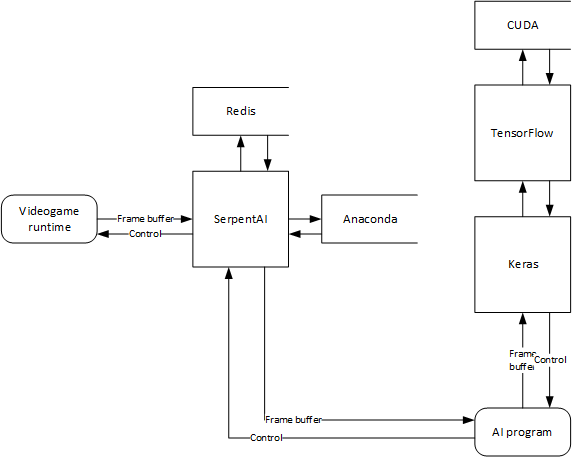
\includegraphics[scale = 0.75]{dataflow.png} \\
\end{figure}

With the replay loader, it is possible to use replays to efficiently train a machine learning model.

%-------------------------------------------%

\section{Frameworks}
%-------------------------------------------%

Our project uses a software stack comprised of the following modules and libraries: SerpentAI, Keras, TensorFlow, and the Anaconda Distribution for Python 3. We chose to use Python 3 as our primary programming language for its flexibility, intuitive syntax, and data processing capabilities. Python is also helpfully compatible with all of the other software listed above. Furthermore, the {\it Anaconda distribution} provides us with a large assortment of Python modules, some of which {\it SerpentAI} cites as dependencies \cite{SerpentAI}. This allows us to more easily work from within a Windows environment, which in turn gives us the most straightforward and stable access to GPU computation via NVIDIA proprietary drivers. TensorFlow serves as the project's backbone by actually creating the neural network in addition to performing the necessary computations \cite{TensorFlow}, with Keras allowing us to perform rapid prototyping in TensorFlow via its abstracted API \cite{Keras}.

All experiments will take place on a pair of 64-bit Windows 10 machines with Ubuntu subsystems. There are several reasons to justify this decision. Firstly, we wanted to ensure that we would have the best possible experience when dealing with GPU computation, and NVIDIA simply has a longer and better track record for supporting Windows than it does for Linux. Secondly, we wanted to avoid the potential pitfall of our platform restricting us to a smaller library of target games. Our two top candidates were Quake and Rivals of Aether because both of these games support replays, or demos; however, of those two games, only Quake natively supports Linux, and ultimately we selected Rivals of Aether. Lastly, and with regards to using our own computers for both development and testing: we made the decision to abstain from distributed or cloud computing chiefly to save costs, but also as an aesthetic choice based in our desire to push our own hardware to its absolute limits. Despite all of the above justifications for using Windows, it remains to be said that our project cannot live without Linux. SerpentAI requires a Redis database, so in order for that to work we use an Ubuntu subsystem; this is the official recommendation from the SerpentAI developers \cite{SerpentAI}.

%-------------------------------------------%



\section{Algorithms}
%-------------------------------------------%

The artificial neural network takes 2 inputs and produces 1 output. These are \textit{x}, \textit{y\textsubscript{1}}, and \textit{y}, respectively.

The primary input, \textit{x}, is of a video clip consisting of 60 gray-scale frames, where each frame is 80 by 45 pixels with 1 color channel. The auxiliary input, \textit{y\textsubscript{1}}, contains the most recent actions taken by the player; these are represented by an array containing 9 integers, where each index of the array is associated with a different action and contains either a 1 if the player took that action or a 0 if not.

The video clips are processed by a stack of four 2D convolutional LSTM layers that are buffered with 2D batch normalization layers. At the same time, the recent actions are fed into a stack of two normal LSTM layers. Next, both stacks are concatenated together. The resulting concatenation is then given to a deep neural network containing RELU activations. Finally, this leads to the output layer, \textit{y\textsubscript{1}}; this layer applies a sigmoid function across 9 nodes, where each node again represents each of the different actions available to the player. In this case, the layer is predicting which actions are about to be taken by the player.

During training and testing, \textit{y\textsubscript{1}} is always the \textit{y} from the previous frame. During live game-play, however, each value from \textit{y} is converted into either 1 or 0 based on a threshold value. The result of this thresholding is then used as the next \textit{y\textsubscript{1}}.

\begin{figure}
    \caption{High-level overview of the neural network}
    \centering
    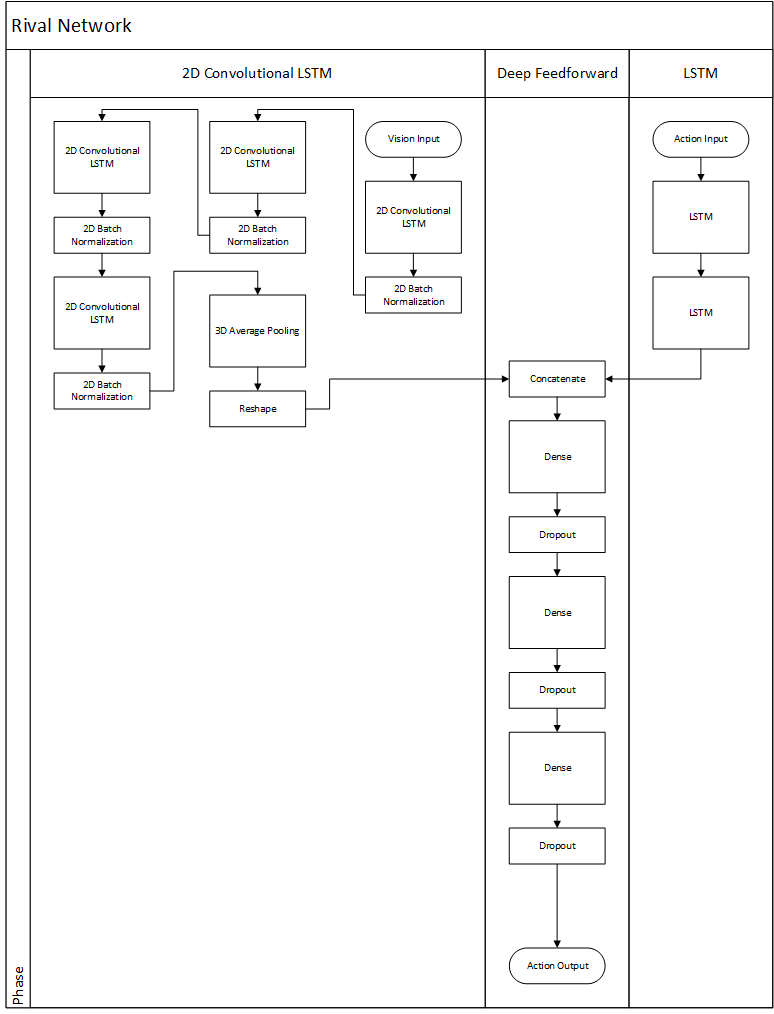
\includegraphics[scale = 0.5]{network.png} \\
\end{figure}

%-------------------------------------------%



\section{Features}
%-------------------------------------------%

In order to play Rivals of Aether, one must use a set of controls containing a total of nine buttons, where five are for actions such as attacking or dodging and four are for movement.

\begin{figure}
	\caption{In-game menu displaying game controls}
	\centering
	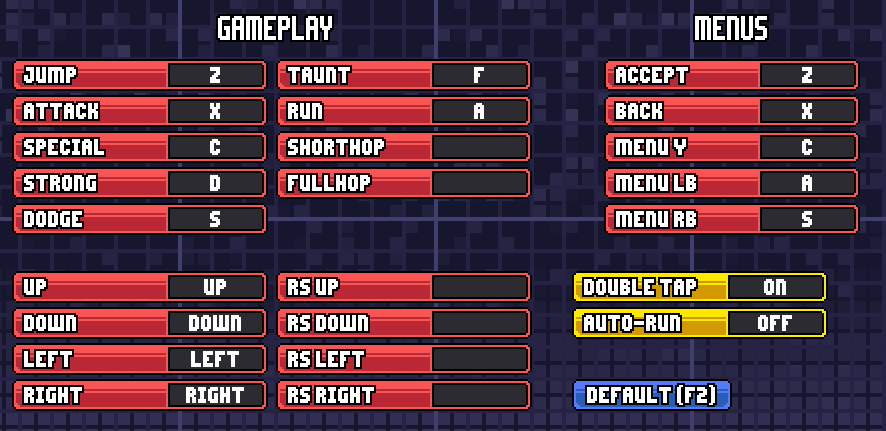
\includegraphics[scale = 0.5]{controls.png} \\
\end{figure}

These buttons can be combined for different effects. An attack will undergo significant changes depending on if the attacking character is standing, walking, running, or jumping. Furthermore, tilting the control stick during the attack will effect additional changes. Dodging in the air is different from doing so on the ground, which is different still from dodging while moving the control stick in a direction.

Due to the complex nature of the game's control scheme, at any given moment the AI will need to be able to output any combination of two simultaneous button presses, where one of the buttons is for movement and the other is for an action.

%-------------------------------------------%



\section{Test Plan}
%-------------------------------------------%

The full dataset contains a total of 1,032 replay files provided by the Rivals of Aether community. Of those, 222 replay files are unusable because they were recorded in pre-release versions of the game that do not appear to normally support replay recording or playback. Given that the replays exist in the first place, it is conceivable that the functionality exists via an undocumented developer menu or console command. No such accesses were found, however. With the unusable 222 replay files removed, the dataset is left with only 810 replays. Leaving out 20 percent of the dataset for testing reduces the training set to a meager 641 replays. This is not as poor as it may seem at first, however. Each replay can have a duration anywhere up to 8 minutes. Thus, with the frame collector running at 10 frames per second, this leads to an upper limit of 4,800 frames sampled per replay. As a result, the training set contains a total of 859,249 frames while the testing set has 221,782.

The amount of data can still be increased, however. Replays contain input data for a minimum of 2 players and a maximum of 4. This one-to-many relation from replays to players can be exploited if each combination of a replay and player is treated as a separate video. In other words, the frame buffer for replay \textit{R} can be used not only with the input data for player \textit{\textit{P\textsubscript{1}}} but also with those of players \textit{P\textsubscript{2-4}}. Exploding the dataset in this fashion yields a total of 1271 replays for training and 332 replays for testing. 

A training session will run as follows. The SerpentAI agent will traverse the game's menus to initiate playback of the next replay from a shuffled copy of the training set. While the match is simulated, the agent will simultaneously read the visual buffer from the game and control input data from the replay file. For each frame, the agent will pair the input data with its corresponding visual buffer and then send this bundle to a TensorFlow neural network as labels and data, respectively. The neural network will attempt to produce a set of appropriate control inputs in response and adjust its weights  whenever its prediction are incorrect. When playback has concluded, the agent will traverse the menus once again to start a new replay, repeatedly, until it has reached its quota. The total number of training iterations will vary between experiments until it produces satisfactory results.

A properly trained neural network shall demonstrate several qualities other than a high accuracy when tested against the held back data. Firstly, it shall be able to defeat low-level in-game bots, thereby demonstrating its competence. This can be tested by placing the neural network in matches against bots of increasing difficulty, thereby enabling the assignment of numerical performance benchmarks. Secondly, it shall play in a believably-human manner. This means that it should, wherever possible, be discouraged from playing {\it inhumanly} well, getting stuck, or displaying mechanical tics. Examples of these undesirable behaviors would include, in order, executing nonstop frame-perfect moves throughout the course of an entire game, running off of the stage or standing still due to an as-of-yet unseen situation, or constantly changing direction for no reason while otherwise playing competently. Identifying all such behaviors will be difficult prior to live experiments, however.

%-------------------------------------------%



\section{Criteria and Constraints}
%-------------------------------------------%

Initial work on the neural network implementation is due to start on December 12, 2017, shortly after the conclusion of the 2017 Fall Semester. This work should be concluded by mid-March. From there, about two weeks are allocated for finalizing the design document. Overall, the schedule is intentionally tight in order to emphasize getting most of the work done in the beginning of the semester, thereby maximizing flex time and minimizing the competition between this project and other finals.

\begin{figure}
	\caption{Gantt chart}
	\centering
	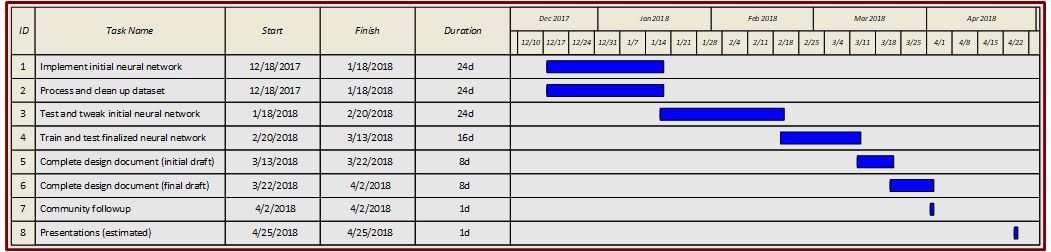
\includegraphics[scale = 0.5]{gantt.png} \\
\end{figure}

The project has other constraints in addition to its schedule. The dataset was collected from the community with the promise that each replay file we receive will be treated as private data and not, under any circumstances, be redistributed. Thus, care shall be taken to ensure that no replay files from the community are leaked. At the same time, however, these files must not be lost due to accidental deletion, disk failure, or lack of backup. To address these requirements, multiple redundant copies of the dataset are stored on our own local drives as well as via encrypted, private, cloud storage services such as Google Drive. Only the dozen or so replay files that we brought to the dataset ourselves may be stored publicly on the GitHub repository.

Our experiments will be deemed adequately successful if we can produce AI that beat the in-built bots on lowest difficulty levels. This is considered a baseline that we will attempt to surpass through improvements to the neural network and additional training.

%-------------------------------------------%
